\documentclass[tikz]{standalone}
\usepackage[mode=buildnew]{standalone}
\usepackage{pgfplots}
\usetikzlibrary{
arrows.meta,
arrows,
calc,
decorations.pathreplacing, 
ext.paths.ortho,
positioning,
quotes,
fit,
external
}
\tikzstyle{line}=[draw]
\begin{document}
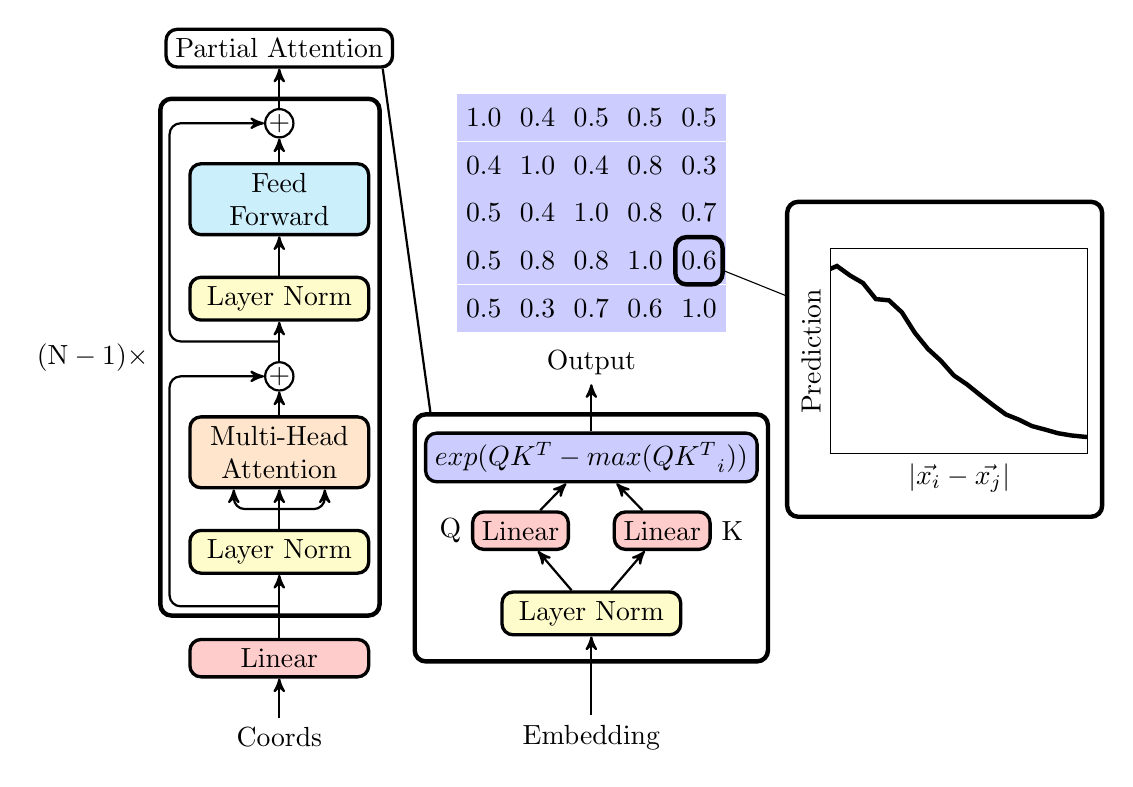
\begin{tikzpicture}[
module/.style={draw, very thick, rounded corners, minimum width=15ex},
embmodule/.style={module, fill=red!20},
mhamodule/.style={module, fill=orange!20},
lnmodule/.style={module, fill=yellow!20},
ffnmodule/.style={module, fill=cyan!20},
pattn_small/.style={module},
pattn/.style={module, fill=blue!20},
arrow/.style={-stealth', thick, rounded corners},
node distance = 0.5cm,
% > = {Stealth[round, sep]}
% x=2cm,
]
% \begin{tikzpicture}[
%   thick, x=2cm, node distance=7.5mm,
%   n/.style={rounded corners, draw, fill={#1!20}},
%   > = {Stealth[round, sep]}]
% \node (inputs) {Inputs};
% % \node[above=of inputs, embmodule, align=center] (inputemb) {Input\\Embedding};
% \node[above=of inputs, embmodule, align=center] (inputemb) {Embedding};
% \node[right=of inputemb, embmodule, align=center] (coordsemb) {Linear};
% \node[below=of coordsemb] (coords) {Coords};
% \node[above=of $(inputemb)!0.5!(coordsemb)$, draw, thick, circle] (embplus){$+$};
% \node[above=of embplus, yshift=0.5cm, mhamodule, align=center] (mha) {Multi-Head\\Attention};
\node (coords) {Coords};
% \node[above=of inputs, embmodule, align=center] (inputemb) {Input\\Embedding};
\node[above=of coords, embmodule, align=center] (coordsemb) {Linear};
\node[above=of coordsemb, yshift=0.3cm, lnmodule, align=center] (norm1) {Layer Norm};
\node[above=of norm1, mhamodule, align=center] (mha) {Multi-Head\\Attention};
% \node[above=of mha, lnmodule, align=center] (addnorm1) {Add \& Norm};
\node[above=of mha, yshift=-0.2cm, inner sep=0, draw, thick, circle] (addnorm1){$+$};
\node[above=of addnorm1, lnmodule, align=center] (norm2) {Layer Norm};
\node[above=of norm2, ffnmodule, align=center] (ffn) {Feed\\Forward};
% \node[above=of ffn, lnmodule, align=center] (addnorm2) {Add \& Norm};
\node[above=of ffn, yshift=-0.2cm, inner sep=0, draw, thick, circle] (addnorm2){$+$};
\node[above=of addnorm2, pattn_small] (outputs) {Partial Attention};
% \node[left=of embplus, draw, thick, circle, inner
% sep=0pt,label={[align=left]left:Positional\\Encoding}]
% (pe) {\tikz \draw[scale=0.1] plot[domain=0.0:6.28]
% (\x,{sin(\x r)});};
% \draw[arrow] (inputs) -- (inputemb);
% \draw[arrow] (inputemb) -- (embplus);
\draw[arrow] (coords) -- (coordsemb);
% \draw[arrow] (coordsemb) -- (embplus);
\draw[arrow] (coordsemb) -- (norm1);
\draw[arrow] (norm1) -- (mha);
% \draw[arrow] (embplus) -- (mha);
\draw[arrow] (mha) -- (addnorm1);
% \draw[arrow] (addnorm1) -- (ffn);
\draw[arrow] (ffn) -- (addnorm2);
\draw[arrow] (addnorm2) -- (outputs);
% (addnorm2) edge (outputs)

% \coordinate (mharesidual) at ($(mha.south)!0.5!(embplus.north)$);
\coordinate (mharesidual) at ($(norm1.south)!0.5!(coordsemb.north)$);
\coordinate (ffnresidual) at ($(norm2.south)!0.5!(addnorm1.north)$);
\coordinate (mhafork) at ($(mha.south)!0.5!(norm1.north)$);
% \coordinate (pafork) at ($(outputs.south)!0.5!(addnorm2.north)$);
\coordinate[left=of addnorm1, xshift=-0.7cm] (ln1residualleft);
\coordinate[left=of addnorm2, xshift=-0.7cm] (ln2residualleft);

\node[fit={(mha)(addnorm2)(mharesidual)(ln1residualleft)}, draw, ultra thick, rounded corners, label=left:$\mathrm{(N-1)\times}$](encoder) {};

\draw[arrow](mharesidual)-|(ln1residualleft)--(addnorm1);
\draw[arrow](ffnresidual)-|(ln2residualleft)--(addnorm2);
\draw[arrow] (mhafork)-|($(mha.south)!0.5!(mha.south west)$);
\draw[arrow] (mhafork)-|($(mha.south)!0.5!(mha.south east)$);
% \draw[arrow] (pafork)-|($(outputs.south)!0.33!(outputs.south west)$);
% \draw[arrow] (pafork)-|($(outputs.south)!0.33!(outputs.south east)$);
\draw[arrow] (addnorm1) -- (norm2);
\draw[arrow] (norm2) -- (ffn);



\node[right=of coords, xshift=1.8cm] (emb) {Embedding};
\node[above=of emb, yshift=0.5cm, lnmodule] (norm3) {Layer Norm};
\node[above=of norm3, xshift=-0.9cm, embmodule, minimum width=5ex, label=left:Q] (lin2) {Linear};
\node[above=of norm3, xshift=0.9cm, embmodule, minimum width=5ex, label=right:K] (lin3) {Linear};

\node[above=of $(lin2)!0.5!(lin3)$, yshift=0.1cm, pattn] (exp) {$exp(QK^T-max({QK^T}_i))$};
\node[above=of exp, yshift=0.1cm] (output) {Output};
\draw[arrow] (emb) -- (norm3);
\draw[arrow] (norm3) -- (lin2);
\draw[arrow] (norm3) -- (lin3);
\draw[arrow] (lin2) -- (exp);
\draw[arrow] (lin3) -- (exp);
\draw[arrow] (exp) -- (output);

\coordinate[yshift=-0.2cm] (pabot) at (norm3.south);
\coordinate[yshift=-0.2cm] (patop) at ($(exp.north)!0.5!(output.south)$);
% \coordinate (mhafork) at ($(mha.south)!0.5!(mharesidual)$);
% \coordinate (pafork) at ($(outputs.south)!0.5!(addnorm2.north)$);
\coordinate[left=of exp, xshift=0.5cm] (paleft);
\coordinate[right=of exp, xshift=-0.5cm] (paright);

\node[fit={(pabot)(patop)(paleft)(paright)}, draw, ultra thick, rounded corners](pa_big) {};

% \draw[style=thick] (outputs) -- (pa_big);
\coordinate[right=of outputs] (pasmallright);
% \draw[style=ultra thick](outputs)-|(pasmallright)--(pa_big.north west);
\coordinate[] (pasmallpt) at ($(outputs.south)!0.9!(outputs.south east)$);
\coordinate[] (pabigpt) at ($(pa_big.north)!0.9!(pa_big.north west)$);
\draw[style=thick](pasmallpt) -- (pabigpt);


\matrix [nodes={fill=blue!20,minimum size=6mm}, above=of output, yshift=-15]
  {
    \node {1.0}; & \node{0.4}; & \node {0.5}; & \node {0.5}; & \node {0.5}; \\
    \node {0.4}; & \node{1.0}; & \node {0.4}; & \node {0.8}; & \node {0.3}; \\
    \node {0.5}; & \node{0.4}; & \node {1.0}; & \node {0.8}; & \node {0.7}; \\
    \node {0.5}; & \node{0.8}; & \node {0.8}; & \node {1.0}; & \node(example) {0.6}; \\
    \node {0.5}; & \node{0.3}; & \node {0.7}; & \node {0.6}; & \node {1.0}; \\
  };
  \begin{axis}[xmin=0,xmax=2, 
  xlabel=$|\vec{x_i}-\vec{x_j}|$,
   ylabel=Prediction,
   samples=100,
   ticks=none,
   ylabel near ticks,
    xlabel near ticks,
  % above=of MHAtt,
  % anchor=center
  at={(70mm,36mm)},
  width=0.4\linewidth,
  ]
  \pgfmathsetseed{3}%
  \addplot[black, ultra thick] (x, {e^(-x*x+0.05*rand)});
\end{axis};
  % node[draw, ultra thick, rounded corners]
  \node[at=(example.center), minimum size=6mm, draw, ultra thick, rounded corners](example_box1) {};
  \node[at={(8.45cm,4.8cm)}, minimum size=40mm, draw, ultra thick, rounded corners](example_box2) {};
  \draw (example_box1) -- (example_box2);

\end{tikzpicture}
\end{document}